% !Tex root = main.tex
\newpage
\section{Theory}
\emph{Functional Dependencies}~(FDs) are a way of expressing ``a priori knowledge of restrictions or constraints on permissible sets of data''~\cite[p.~42]{MAI83} in relational database theory.
Having been introduced in the 1970s for schema normalization of relational databases, FDs have proven to be useful in a multitude of domains. In this section, \emph{functional dependencies} and the theoretical foundation necessary to put them into context are introduced.

\subsection{Relational Database Theory}
In order to give a definition of FDs, they need to be put in context to the domain they stem from: relational database theory. Some basic concepts will be introduced in this section.

\subsubsection{Relation Scheme}
A \emph{relation scheme}\footnote{also called \emph{relational schema} in literature\cite[p.21]{ABE19} } \(\boldsymbol{R}\) is a finite set of \emph{attribute names} \(\{A_1,~A_2,~\dots,~A_n\}\), where to each attribute name \(A_i\) corresponds a set \(D_i\), called \emph{domain} of \(A_i\), \(1 \leq i \leq n\).
Let \(\boldsymbol{D}~=~D_1 \cup D_2 \cup \dots \cup D_n$, then a \emph{relation} \(r\) on relation scheme \(\boldsymbol{R}\) is a finite set of mappings \(\{t_1, t_2, \dots, t_p\}\) from \(\boldsymbol{R}\) to \(\boldsymbol{D}\):
\begin{align*}
  &t_i: \boldsymbol{R} \to \boldsymbol{D},
\end{align*}
where we call those mappings \emph{tuples} under the constraint that~\cite[p.2]{MAI83}
\begin{align*}
    t(A_i) \subseteq D_i.
\end{align*}
In application, attribute names are commonly called \emph{column name} or \emph{column attribute}.
One can think of them as labels of data that is stored in the respective column.


\subsubsection{Keys}
A \emph{key} on a relation \( r \) on a relation scheme \( R \) is a subset \( K = \{ B_1, B_2, \dots, B_m \} \) with the property that for any tuple \( t_i \in \{ t_1, t_2, \dots, t_3 \} \) the relation
\begin{align*}
    t_i(B_k) = t_j(B_k) \Rightarrow t_i \equiv t_j
\end{align*}
holds for any single \( B_k \in K \). In other words, any \( K \)-value of a tuple identifies that tuple uniquely.~\cite[p.~4]{MAI83}

Having defined both \emph{relation scheme} and \emph{keys}, it is now possible to introduce the more complex concepts of relational databases and functional dependencies.


\subsubsection{Definition of a Relational Database}
When real-world data used by one or multiple application/s is stored on a machine according to the relational model, it is usually stored in a relational database.
According to the definition of a relation scheme \(R\), one can formally introduce databases and database schemes:

We assume that \(R\) is composed of two parts, \(S\) and \(\boldsymbol{K}\). We call \(S\) a \emph{set of attributes} and \(\boldsymbol{K}\) a \emph{set of designated keys} and describe this composition by writing \(R = (S, \boldsymbol{K})\).
A \emph{relational database scheme} \textbf{R} over \textbf{U} can now be defined as a collection of relation schemes \(\{R_1, R_1, \dots, R_p\}\), where \(R_i = (S_i, \boldsymbol{K}_i)\), \(1 \leq i, j \leq p\),
\begin{align*}
    \bigcup^{p}_{i=1} S_i = \boldsymbol{U}.
\end{align*}
We demand that \(S_i \neq S_j\) if \(i \neq j\).

A \emph{relational database} \( d \) on a \emph{database scheme} \textbf{R} is a collection of relations \( d~=~\{r_1, r_2, \dots, r_p \} \) such that for each relation scheme \(R = (S, \boldsymbol{K}) \) in \textbf{R} there is a relation \(r\) in \(d\) such that \(r\) is a relation on \(S\) that satisfies every \emph{key} in \(\boldsymbol{K}\).~\cite[p.~94]{MAI83}


\subsubsection{Definition of a Functional Dependency}
Consider a relation \(r\) on scheme \(\boldsymbol{R}\) with subset \(X \subseteq \boldsymbol{R}\) and a single attribute \(A_i \in \boldsymbol{R}\).
A FD \(X \to A\) is said to be \emph{valid} in \(r\), if and only if
\begin{align}
    t_i[X] = t_j[X] \Rightarrow t_i[A] = t_j[A] \label{eq:fd-condition}
\end{align}
holds for all all pairs of distinct tuples \(t_i,t_j \in r\).\cite[p.~21]{ABE19}
We say that \(X\) \emph{functionally determines} \(A\)\cite[p.~43]{MAI83} and name \(X\) the \emph{left hand side} (lhs), whilst calling \(A\) the \emph{right hand side} (rhs).

\begin{table}[ht]
    \centering
    \begin{tabular}{rlllr}
        \toprule
        & \multicolumn{3}{c}{left hand side} & \multicolumn{1}{c}{right hand side} \\ \cmidrule(lr{.25em}){1-4} \cmidrule(l{4.75em}){4-5}
        \textsc{Id} & \textsc{Prename} & \textsc{Surname} & \textsc{Town} & \textsc{Zip} \\
        \midrule
        1 & Alice & Smith & Munich & 19139 \\
        2 & Peter& Meyer & Munich & 19139 \\
        3 & Ana & Parker & Munich & 19139  \\
        4 & John & Pick & Berlin & 12055 \\
        5 & John & Pick & Munich & 19139 \\
        \bottomrule
    \end{tabular}
    \caption{Example for a FD.}\label{tab:fd-example}
\end{table}

Considering table~\ref{tab:fd-example}, one can see that every tuple in the \emph{left hand side} subset of the relation uniquely determines the \emph{right hand side}.
For the given example we say that \textsc{Id}, \textsc{Prenameame}, \textsc{Surname}, \textsc{Town} \emph{functionally determines} \textsc{Zip}, or \{\textsc{Id}, \textsc{Prename}, \textsc{Surname}, \textsc{Town}\} \( \rightarrow \) \textsc{Zip}.~\cite[p.~43]{MAI83}

If inspected closely, one can discover even more FDs in table~\ref{tab:fd-example}.
For example, \textsc{Town}~\( \rightarrow \)~\textsc{Zip} and \textsc{Id}~\( \rightarrow \)~\textsc{Zip}.
Since \textsc{Town} and \textsc{Id} are subsets of \{\textsc{Id},~\textsc{Prename},~\textsc{Surname},~\textsc{Town}\}, we call \{\textsc{Id},~\textsc{Prename},~\textsc{Surname},~\textsc{Town}\} \emph{non-minimal}.
A FD X~\( \rightarrow \)~A is \emph{minimal}, if no subset of X functionally determines A.~\cite[p.~2]{PAP15}
Thus, \textsc{Id}~\( \rightarrow \)~\textsc{Zip} and \textsc{Town}~\( \rightarrow \)~\textsc{Zip} are \emph{minimal FDs}.

\section{FDs in Application}
FDs are primarily used in database normalization,\cite[p.~1]{CAR16} but also find application in the field of data profiling, where ``any dependency can be turned into a rule to check for errors in the data''.\cite[p.~9]{ABE19}

\subsection{Normalization}
When introducing the relational database model in his 1970 article ``A relational model of data for large shared data banks'', Edgar F. Codd formalized database normalization alongside.\cite{COD70}
Describing what will be know to academia as \textbf{First normal form} (1NF), Codd states that ``problems treated [when normalizing databases] are those of \emph{data independence}'', aiming to protect future users of large databases ``from having to know how the data is organized in the machine''. \cite[p.~1]{COD70}

Being designed for as efficient as possible query handling, databases at the time were structured hierarchically or navigationally.
While this yielded good performance in times when computing time was very expensive, it came with a heavy cost of complexity:
``Teams of programmers were needed to express queries to extract meaningful information. [\dots] Such databases [\dots] were absolutely inflexible[y]''.\cite{IBM03}

Update-, insertion- and deletion anomalies can be prevented when normalizing a relational database. \cite[p.~75]{KLE11}

\subsubsection{First Normal Form}
A relation scheme $R$ is in \emph{First Normal Form} (1NF), if values in \(dom(A)\) are atomic for every attribute \(A\) in \(R\). \cite[p.~96]{MAI83}
Consider table~\ref{tab:first-normal-form} which represents two relational database schemes.
It serves as an example of what is called \emph{atomic} and \emph{compound} data in the Relational Database model. \cite[p.~6]{COD90}

\begin{table}[ht]
    \centering
    \ra{1.3}
    \begin{tabular}{@{}rlllllll@{}}\toprule
    & \multicolumn{3}{c}{Compound Scheme} & \phantom{abc}& \multicolumn{2}{c}{Atomic Scheme} \\
    \cmidrule{2-3} \cmidrule{5-8}
    & \textsc{Name} & \textsc{Adress} && \textsc{Prename} & \textsc{Surname} & \textsc{Town} & \textsc{Street}   \\ \midrule
    1 & Alice Smith & Munich, Alicestr. && Alice & Smith & Alicestr. & Munich \\
2 &  Peter Meyer & Munich, Peterstr. && Peter & Meyer & Munich & Peterstr. \\
3 & Ana Parker & Munich, Anastr. && Ana & Parker & Munich & Anastr. \\
4 & John Pick & Berlin, Johnstr. && John & Pick & Berlin & Johnstr. \\
\bottomrule
\end{tabular}
\caption{The compound attributes \textsc{Adress} and \textsc{Name} can be split into their atomic components \textsc{Town} and \textsc{Street} as well as \textsc{Prename} and \textsc{Surname}, respectively.}\label{tab:first-normal-form}
\end{table}
While the compound scheme's attributes can be decomposed into several other attributes, whereas an atomic attribute cannot be further split into any meaningful smaller components.

For a database it is said that the database in 1NF if every relation scheme in the database scheme is in 1NF.
1NF is the very foundation of the Relational Model, where the only type of compound data is the relation.\cite[p.~6]{COD90}

\subsubsection{Second Normal Form (2NF)}
A relation scheme \(R\) is said to be in \emph{second normal form} (2NF) in respect to a set of FDs \(F\), if it is in 1NF and every nonprime attribute is fully dependent on every key of of \(R\).\cite[p.~99]{MAI83} This definition can be extended for databases: A database scheme \textbf{R} is in second normal form with respect to \(F\) if every relation scheme \(R\) in \textbf{R} is in 2NF with respect to \(F\).

\subsubsection{Third Normal Form (3NF)}


\subsection{Approximate Functional Dependencies}
In the field of data profiling an extensive body of theory and algorithms for FD detection has been created in the past decades.\cite{PAP15}
These mainly consider FDs as defined in formula \ref{eq:fd-condition}.
Howevever, the strict detection of FDs yields results that are solely applicable in a strictly controlled environment.
Real-world datasets faced by data-scientists or database engineers are often \emph{noisy}.
Entries might be corrupted by missing data, wrongly entered entries or incomplete datasets.
Inconsistencies are to be expected.
Thus, functionally dependent column-combinations might not be detected as such. This may result in misleading insights when searching for FDs.

To illustrate this, table \ref{tab:example-afd-necessity} shows an example of noisy data.
The potential FD \textsc{Town} \(\to\) \textsc{\textsc{Zip}} is not captured by the definition given in equation \ref{eq:fd-condition}.
Due to a type-error, the potential FD is invalidated.
To still capture meta-information, a different dependency-measure than given in equation \ref{eq:fd-condition} is needed.

\emph{Approximate FDs} (AFDs), sometimes called \emph{Relaxed FDs}, improve the applicability of FDs, ``in that they relax one or more constraints of the canonical FDs''\cite[p.~1]{CAR16}. While there are AFDs introducing general error measures, others are defined ``aiming to solve specific problems''\cite[p.~1]{CAR16}.

\begin{table}[ht]
    \centering
    \begin{tabular}{lcccc}
        \toprule
        & \multicolumn{3}{c}{Data} \\ \cmidrule(lr){2-5}
        \textsc{Id} & First name & Last name & Town & \textsc{Zip} \\
        \midrule
        1 & Alice & Smith & Munich & 19139 \\
        \textbf{2} & \textbf{Peter}& \textbf{Meyer} &
        \textbf{Muinch} & \textbf{19139} \\
        3 & Ana & Parker & Munich & 19139  \\
        4 & John & Pick & Berlin & 12055 \\
        \bottomrule
    \end{tabular}
    \caption{Even though column \textsc{Zip} functionally determines column \textsc{Town} (and vice-versa), a FD is not capable of displaying this fact~-~a typing error invalidates the FD.}
    \label{tab:example-afd-necessity}
\end{table}

The error measure for this is not trivial at all. While F1-measures can be established for non-categorical cases, comparing results for different data-types tricky.

\subsection{FD Imputer}
The FD Imputer imputes the column of a table of a relational database.
Empirical Risk Minimization strategies are used to do this.
The table is first split in train-set and validation-set.
Then, FDs are detected on the train-set using HyFD.\cite{PAP16}
Having identified all FDs on the train-set, FD Imputer can impute values of any right-hand side of a particular FD:
This is done by executing an SQL join clause.
FD imputer performs an inner join on all left-hand side columns, joining train-set and validation-set.
A second left join clause concatenates the original validation-set with the column of imputed tuples stemming from the first join.
\begin{algorithm}[H]
    \DontPrintSemicolon
    \SetAlgoLined
    \KwResult{Validation-subset of a relational database table with an additional column containing imputed tuples}
    \KwData{Relational database table}
    \BlankLine

    Split relational database table into train-set and validation-set\;
    Detect FDs in train-set\;
    ALTER TABLE train-set DROP COLUMN not in lhs\;
    imputed-set = SELECT lhs FROM train-set INNER JOIN validation-set ON lhs\;
    imputed-validation-set = SELECT imputed-column FROM imputed-set LEFT JOIN validation-set\;
    return imputed-validation-set\;
    \caption{FD Imputer}
\end{algorithm}


\newpage
\subsection{Machine Learning Classifier Theory}
Once a model has been trained and validated, it needs to be tested in order to determine whether or not overfitting occured during training.
This is usually done by measuring the model's performance on a separate dataset not involved in training, the so called test set.
Performance is measured according to the type of data and the kind of model involved.
To visualize the performance of a classifier, a \emph{confusion matrix} can be created.
\begin{figure}[h]
     \centering
     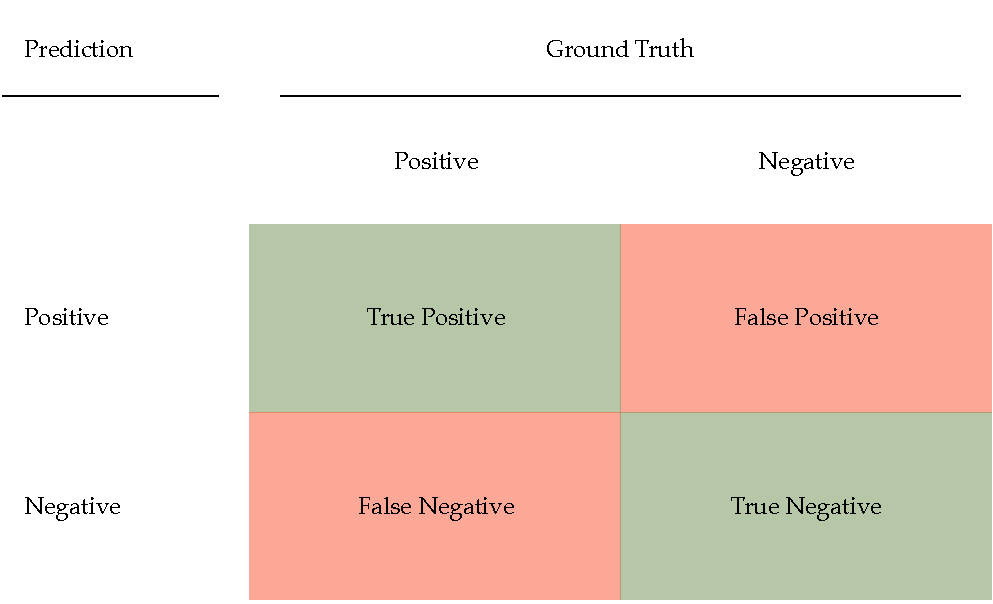
\includegraphics[width=.8\textwidth]{images/binary-confusion-matrix.pdf}
     \caption{Illustration of a binary confusion matrix.
     ``Prediction'' refers to predicted labels \(y_{pred}(x)\) while ``Ground Truth'' represents the actual labels \(y(x)\).}
     \label{fig:confusion-matrix}
 \end{figure}

The simplest case of a confusion matrix can be created when measuring the performance of a binary classifier.
Figure~\ref{fig:confusion-matrix} shows such a binary confusion matrix.
Here, ``Ground Truth'' describes the label \(y(x)\) of some data point \(x \in X_{test}\), where \(y \in \{0, 1\}\).
``Prediction'' identifies the predicted labels \(y_{pred}(x)\) that the model generates after is has been executed on the test-set \(X_{test}\) prior unknown.

Whenever \(y_{pred}(x) = y(x),~x \in X_{test}\) holds, the predicted label can be assigned to be either a \emph{True Positive} (TP) or a \emph{True Negative} (TN).
The opposite holds as well, such that a falsely predicted label will be either a \emph{False Negative} (FN) or a \emph{False Positive} (FP).

Using the classification introduced by the binary confusion matrix, all predicted labels \(y_{pred}\) are assigned to the four sets TP, TN, FN and FP.
Using these four sets, we can introduce measures for classification performance.

\emph{Precision} is a measure that depicts the proportion of correctly classified positive samples to the total amount of samples classified as positive.\cite[p.4]{THA18} This can be algebarically expressed as
\begin{align}
    Precision = \frac{|TP|}{|TP| + |FP|}
\end{align}
where \(|A|\) is the cardinality of a set \(A\). Precision measures how many elements classified as positive are True Positives.

\emph{Recall}, also called \emph{sensitivity}, represents the
share of positive correctly classified samples to the total amount of positive samples.\cite[p.3]{THA18} This can be formalized as
\begin{align}
    Recall = \frac{|TP|}{|TP| + |FN|}
\end{align}
Recall measures how many of the positive labelled elements were actually selected.

\begin{figure}[h]
    \centering
    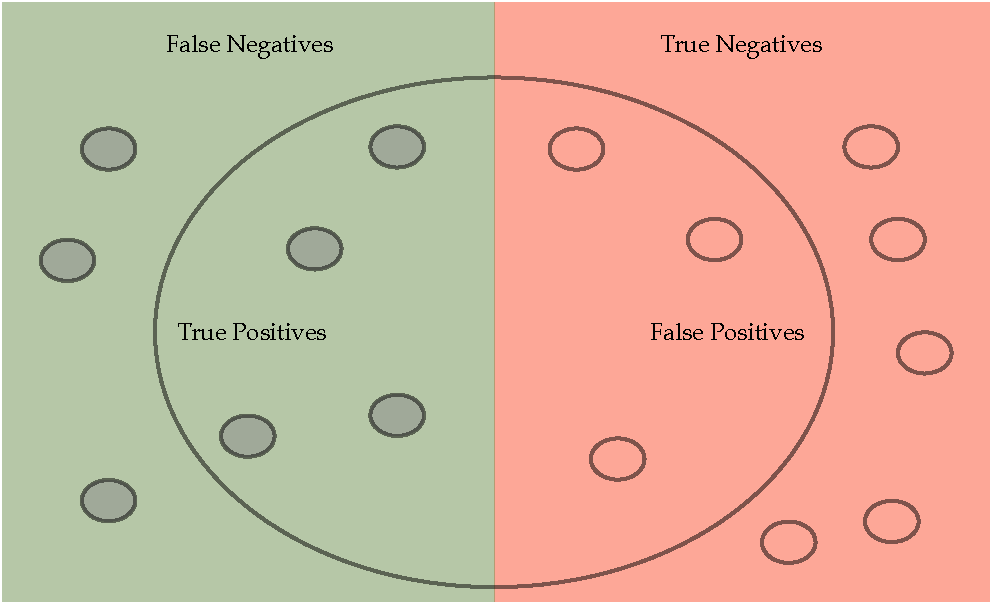
\includegraphics[width=.5\textwidth]{images/precision-and-recall}
    \caption{Each predicted label \(y_{x}\) is represented by a circle. Hollow circles stand for negative labels and full circles for positive lables.  }
    \label{fig:precision-and-recall}
\end{figure}

The harmonic mean of precision and recall is called \emph{F1-measure}:
\begin{align}
F1-measure = {\left(\frac{Recall^{-1} + Precision^{-1}}{2}\right)}^{-1}
\end{align}

\subsection{Datawig Imputer}
Datawig Imputer is an imputation method based on \emph{supervised learning}.
In supervised learning, observations are a set of tuples \( \{\left(\mathbold{x}_1, y_1\right),\left(\mathbold{x}_2, y_2\right), \dots \} \).
We call \( \mathbold{x}_i \in \mathbb{F}\) \emph{feature-vector} in a \emph{feature-space} \( \mathbb{F} \subseteq \mathbb{R}^{n} \) and \( y_i \in S \) \emph{output-attributes} or \emph{labels}.\cite[p.19]{DUD00}

Datawig Imputer solves a classification problem.
A function
\begin{align}
    f: \mathbb{F} \rightarrow S
\end{align}
is being approximated, where \( \mathbb{F} \) is the feature-space and \( S = \{a_1, a_2, \dots, a_M \} \) is a set of attributes.

Datawig Imputer assumes that the column to be imputed, the so-called \emph{label comumn}, contains data that can be transform to obtain attributes \( a_1, \dots, a_M \).\cite[p.2]{BIE18}
All columns on a database table that are \emph{not} the label column are called \emph{feature columns}.
These feature columns are what Datawig Imputer will transform to obtain feature-vectors.

The transformation performed to obtain learnable data assign to the \texttt{string} data of each column \( c \) a numerical representation \( x^c \).
These functions are called \emph{encoders}.
Datawig Imputer separates data into two categories: \emph{categorical data} and \emph{sequential data}.
Different encoders are chosen to transform \emph{categorical data} and \emph{sequential data}.

Categorical data are data that consist of \emph{categorical variables}.
``A categorical variable places a case into one of serveral groups of categories,'' define Moore et al.~\cite[p.~4]{MOO11}.
An example-column \( c_{cat} \) containing categorical variables can be representend by the following set of colors:
\begin{align}\label{eq:c-cat}
    c_{cat} = \{ \texttt{blue},~\texttt{red},~\texttt{yellow},~\texttt{blue},~\texttt{blue},~\texttt{red} \}
\end{align}
Datawig Imputer creates a histogram of column \( c \) and uses the histogram's index \( x^c \in \{1, 2, \dots, M_c \} \) to generate a numerical representation.
\begin{figure}[h]
    \centering
    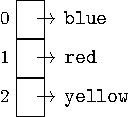
\includegraphics[width=.3\textwidth]{images/state_diagrams/color_histogram}
    \caption{State diagram showing the histogram established by Datawig Imputer to encode example~\ref{eq:c-cat}}
    \label{fig:state-diagram-color}
\end{figure}
Thus the encoded column \( c_{cat} \) would have the following form:
\begin{align}
    c_{cat}^{c} = \{ 0, 1, 2, 0, 0, 1\}
\end{align}

Sequential data is data where the sequece in which individual datapoints are stored in contains information.
An example for sequential data would be a column containing non-categorical strings, like Usernames:
\begin{align}
    c_{seq} = \{ \texttt{ItalyPaleAle},~\texttt{sisou},~\texttt{primos63} \}
\end{align}
The numerical representation \( c_{seq}^{c} \in \{ 0, 1, 2, \dots, A_c \}^{S_c} \) of the sequential column ``is a vector of length \( S_c \), where \( S_c \) denotes the length of the sequence or \texttt{string} in column \( c_{seq} \).''\cite[p.2020]{BIE18}
\( A_c \) denotes the cardinality of the set of all unique characters observed in \( c \).

The histogram created to encode \( c_{seq} \) can be seen in figure \ref{fig:state-diagram-username}.
\begin{figure}[h]
    \centering
    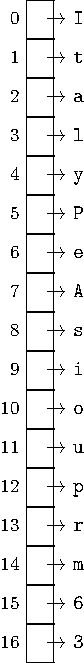
\includegraphics[width=.1\textwidth]{images/state_diagrams/username_histogram}
    \caption{State diagram showing the histogram established by Datawig Imputer to encode \( c_{seq} \).}
    \label{fig:state-diagram-username}
\end{figure}
For \( c_{seq} \), the cardinality of the set of all unique characters is 17.

